\documentclass[11pt,a4paper]{article}
\usepackage[utf8]{inputenc}
%\usepackage{fourier}
\usepackage[english]{babel}
\usepackage{xargs}
\usepackage[pdftex,dvipsnames]{xcolor}
\usepackage{amsmath, amsthm, amssymb, amsfonts}
\usepackage{tablefootnote}
\usepackage{enumerate}
\usepackage{graphicx}
\usepackage{fancyhdr}
\usepackage{booktabs}
\usepackage{epstopdf}
\usepackage{floatrow}
\usepackage{float}
\usepackage[colorlinks=true,breaklinks=false,urlcolor=black,citecolor=red]{hyperref}
\usepackage{listings}
\usepackage[norelsize,ruled,vlined]{algorithm2e}
\usepackage{csquotes}
\usepackage{url}
\usepackage{ifthen}
\usepackage{etoolbox}
\usepackage{datetime}
\usepackage{eurosym}
\usepackage{tikz}
\usepackage[backend=bibtex, backref=true, sorting=none]{biblatex}
\usepackage{caption}

\usepackage{blindtext}
\usepackage{paralist}             % in-paragraph lists
\usepackage{stmaryrd}             % llbracket / rrbracket
\usepackage[nounderscore]{syntax} % grammars
\usepackage{mathtools}
\usepackage[colorinlistoftodos,prependcaption,textsize=tiny]{todonotes}
\usepackage{chngcntr}

\usepackage{datatool}
\usepackage{tabularx}
\usepackage{csvsimple}

\usepackage{highlighter}
\usepackage{qtree} 				% For AST
\usepackage[title]{appendix}



\theoremstyle{definition}
\newtheorem{definition}{Definition}[section]

\theoremstyle{remark}
\newtheorem*{remark}{Remark}

%\counterwithin*{equation}{section}
%\counterwithin*{equation}{subsection}

\newcommand\numberthis{\addtocounter{equation}{1}\tag{\theequation}}

\newcommand{\slang}{\textit{SLang}}
\newcommand{\nullable}{\textit{$@$Nullable}}

\DeclareCaptionFont{white}{\color{white}}

\DeclareCaptionFormat{listing}{\colorbox[cmyk]{0.43, 0.35, 0.35,0.01}{\parbox{\textwidth-\itemindent-2\fboxsep}{\hspace{12pt}#1#2#3} } }

\DeclareCaptionFormat{listingEnum}{\colorbox[cmyk]{0.43, 0.35, 0.35,0.01}{\parbox{\textwidth-\leftmargin-\itemindent-2\fboxsep}{\hspace{12pt}#1#2#3}}}

\captionsetup[lstlisting]{format=listing, labelfont=white, textfont=white, singlelinecheck=false, margin=0pt, font={bf,footnotesize} }


\addbibresource{thesis.bib}
\renewcommand{\baselinestretch}{1.1}

\widowpenalty10000
\clubpenalty10000

%%%%%%%%%%%%%%%%%%%%%%%%%%%%%%%%%%%%%%%%%%%%%%%%%%%%%%%%%%%%%
%                        Setup
%%%%%%%%%%%%%%%%%%%%%%%%%%%%%%%%%%%%%%%%%%%%%%%%%%%%%%%%%%%%%

\begin{document}
\normalfont

\definecolor{dkgreen}{rgb}{0,0.6,0}
\definecolor{gray}{rgb}{0.5,0.5,0.5}
\definecolor{mauve}{rgb}{0.58,0,0.82}
\definecolor{pgrey}{rgb}{0.46,0.45,0.48}

\lstdefinestyle{scala}{
  %captionpos=b,   
  language=Scala,
  aboveskip=3mm,
  basicstyle=\small\ttfamily,
  belowskip=3mm,
  breakatwhitespace=false,
  showspaces=false,
  showlines=true,
  columns=flexible,
  keepspaces=true,
  commentstyle=\color{dkgreen},
  keywordstyle=\color{blue},
  numbers=left,
  numberstyle=\tiny\color{gray},
  showstringspaces=false,
  stepnumber=1,
  extendedchars=true,
  literate={Ⲕ}{{$\kappa$}}1 {⊢}{{$\vdash$}}1,
  moredelim=[is][\textcolor{pgrey}]{\%\%}{\%\%}
}



\definecolor{dkgreen}{rgb}{0,0.6,0}
\definecolor{gray}{rgb}{0.5,0.5,0.5}
\definecolor{mauve}{rgb}{0.58,0,0.82}

\lstset{language=Scala,
  aboveskip=3mm,
  basicstyle={\small\ttfamily},
  belowskip=3mm,
  breakatwhitespace=true,
  breaklines=true,
  columns=flexible,
  commentstyle=\color{dkgreen},
  keywordstyle=\color{blue},
  numbers=left,
  numberstyle=\tiny\color{gray},
  showstringspaces=false,
  stepnumber=1,
  stringstyle=\color{mauve},
  tabsize=2,
}
\lstset{style=scala}

\usetikzlibrary{calc,trees,positioning,arrows,chains,shapes.geometric,%
    decorations.pathreplacing,decorations.pathmorphing,shapes,%
    matrix,shapes.symbols}
\tikzset{>=stealth',
  punktchain/.style={rectangle,
    rounded corners,
    % fill=black!10,
    draw=black, very thick,
    text width=12.5em,
    minimum height=2.5em,
    text centered,
    on chain},
  every join/.style={->, shorten >=2pt},
}


% Example of title page for the projects carried out within the lasec

% Simply include it in your mastex tex file:
%        % Example of title page for the projects carried out within the lasec

% Simply include it in your mastex tex file:
%        % Example of title page for the projects carried out within the lasec

% Simply include it in your mastex tex file:
%        \input{cover}


% Updated March 2006 (SP)


\newcommand{\logoepfl}[0]{
  \begin{center}
    
\includegraphics[width=4cm]{logo_epfl_coul.pdf}
  \end{center}
  \vspace{0.3cm}
  \hrule
}
\newcommand{\logolasec}[0]{
  \vspace{1cm}
  \hrule
  \begin{center}
    \includegraphics[width=4.5cm]{logo_lasec_coul.eps}
  \end{center}
}
\newcommand{\project}[1]{
  \begin{center}
    \large{#1}
  \end{center}
  \vspace{1cm}
}
\newcommand{\department}[1]{
  \begin{center}
    \large{#1}
  \end{center}
}
\newcommand{\supervisor}[3]{
  \begin{center}
    \begin{normalsize}{
        \bf #1}\\#2\\#3
    \end{normalsize}
  \end{center}
}
\renewcommand{\author}[1]{
  \begin{center}
    \Large{#1}
  \end{center}
  \vspace{0.5cm}
}
\renewcommand{\title}[1]{
  \vspace{3cm}
  \begin{center}
    \huge{#1}
  \end{center}
  \vspace{1.7cm}
}
\renewcommand{\date}[2]{
  \begin{center}
    \normalsize{#1 #2}
  \end{center}
  \vspace{0.5cm}
}


\thispagestyle{empty}


% begin title page
  \logoepfl

  \title{Using an universal intermediate representation to perform static analysis}

  \author{Quentin Jaquier}
  \department{School of Computer and Communication Sciences}
  \project{A thesis submitted for the degree of Master of Computer Science at École polytechnique fédérale de Lausanne}

  \date{March}{2019}

  \begin{center}
    \begin{tabular}{ccc}
      \begin{tabular}{p{3.0cm}}
        \supervisor{Supervisor}{Prof. Viktor Kuncak}{EPFL / LARA}
      \end{tabular}&
      \begin{tabular}{p{3.0cm}}
        \supervisor{Company Supervisor}{Dinesh Bolkensteyn}{SonarSource}
      \end{tabular}
    \end{tabular}
  \end{center}

% end title page




% Updated March 2006 (SP)


\newcommand{\logoepfl}[0]{
  \begin{center}
    
\includegraphics[width=4cm]{logo_epfl_coul.pdf}
  \end{center}
  \vspace{0.3cm}
  \hrule
}
\newcommand{\logolasec}[0]{
  \vspace{1cm}
  \hrule
  \begin{center}
    \includegraphics[width=4.5cm]{logo_lasec_coul.eps}
  \end{center}
}
\newcommand{\project}[1]{
  \begin{center}
    \large{#1}
  \end{center}
  \vspace{1cm}
}
\newcommand{\department}[1]{
  \begin{center}
    \large{#1}
  \end{center}
}
\newcommand{\supervisor}[3]{
  \begin{center}
    \begin{normalsize}{
        \bf #1}\\#2\\#3
    \end{normalsize}
  \end{center}
}
\renewcommand{\author}[1]{
  \begin{center}
    \Large{#1}
  \end{center}
  \vspace{0.5cm}
}
\renewcommand{\title}[1]{
  \vspace{3cm}
  \begin{center}
    \huge{#1}
  \end{center}
  \vspace{1.7cm}
}
\renewcommand{\date}[2]{
  \begin{center}
    \normalsize{#1 #2}
  \end{center}
  \vspace{0.5cm}
}


\thispagestyle{empty}


% begin title page
  \logoepfl

  \title{Using an universal intermediate representation to perform static analysis}

  \author{Quentin Jaquier}
  \department{School of Computer and Communication Sciences}
  \project{A thesis submitted for the degree of Master of Computer Science at École polytechnique fédérale de Lausanne}

  \date{March}{2019}

  \begin{center}
    \begin{tabular}{ccc}
      \begin{tabular}{p{3.0cm}}
        \supervisor{Supervisor}{Prof. Viktor Kuncak}{EPFL / LARA}
      \end{tabular}&
      \begin{tabular}{p{3.0cm}}
        \supervisor{Company Supervisor}{Dinesh Bolkensteyn}{SonarSource}
      \end{tabular}
    \end{tabular}
  \end{center}

% end title page




% Updated March 2006 (SP)


\newcommand{\logoepfl}[0]{
  \begin{center}
    
\includegraphics[width=4cm]{logo_epfl_coul.pdf}
  \end{center}
  \vspace{0.3cm}
  \hrule
}
\newcommand{\logolasec}[0]{
  \vspace{1cm}
  \hrule
  \begin{center}
    \includegraphics[width=4.5cm]{logo_lasec_coul.eps}
  \end{center}
}
\newcommand{\project}[1]{
  \begin{center}
    \large{#1}
  \end{center}
  \vspace{1cm}
}
\newcommand{\department}[1]{
  \begin{center}
    \large{#1}
  \end{center}
}
\newcommand{\supervisor}[3]{
  \begin{center}
    \begin{normalsize}{
        \bf #1}\\#2\\#3
    \end{normalsize}
  \end{center}
}
\renewcommand{\author}[1]{
  \begin{center}
    \Large{#1}
  \end{center}
  \vspace{0.5cm}
}
\renewcommand{\title}[1]{
  \vspace{3cm}
  \begin{center}
    \huge{#1}
  \end{center}
  \vspace{1.7cm}
}
\renewcommand{\date}[2]{
  \begin{center}
    \normalsize{#1 #2}
  \end{center}
  \vspace{0.5cm}
}


\thispagestyle{empty}


% begin title page
  \logoepfl

  \title{Using an universal intermediate representation to perform static analysis}

  \author{Quentin Jaquier}
  \department{School of Computer and Communication Sciences}
  \project{A thesis submitted for the degree of Master of Computer Science at École polytechnique fédérale de Lausanne}

  \date{March}{2019}

  \begin{center}
    \begin{tabular}{ccc}
      \begin{tabular}{p{3.0cm}}
        \supervisor{Supervisor}{Prof. Viktor Kuncak}{EPFL / LARA}
      \end{tabular}&
      \begin{tabular}{p{3.0cm}}
        \supervisor{Company Supervisor}{Dinesh Bolkensteyn}{SonarSource}
      \end{tabular}
    \end{tabular}
  \end{center}

% end title page


\begin{abstract}
Statically finding bugs that can arise in production is typically known as a complex process, that is often specific to a single programming language, leading to a non-trivial implementation with specialized data-structures.
Powerful analysis tools already exists, but only for a subset of all existing languages.
Supporting new language requires to re-implements the same checks again and again.
Ideally, we would want to reduce the cost by re-using the same implementation of the checker.
To solve this problem, SonarSource, a company performing static analysis, have introduce an incomplete universal intermediate representation, called \slang{}.
In this work, we are going to try to understand, consolidate, and improve the use of this universal representation to perform static analysis.
\end{abstract}

\section*{Acknowledgement}
\label{sec:acknowledgements}

I would like to express my sincerest gratitude to Professor Viktor Kuncak for supervising my project.
\newline
\newline
Dinesh Bolkensteyn and Marcelo Sousa for their guidance and advice each week throughout this project.
\newline
\newline
And all the members of SonarSource, friends and family who have directly or indirectly guided me in this work.
{
\hypersetup{linkcolor=black}

\tableofcontents
\pagebreak
\lstlistoflistings
\pagebreak
%\listofalgorithms
\listoffigures
\listoftables
}

\setlength{\parskip}{1em}
\section{Introduction}
\label{sec:Introduction}
\section{Adding a new language to SLang}
\label{sec:new_language}

In this part, we are going to discuss the challenge to add a new language to \slang{}, with a general process and a concrete example with \emph{Scala}.

\subsection{General Process}
\label{subsec:general_procedure}

The addition of a new language follows a general process that can be described in a high-level way.
The first step is to choose a front-end to perform the parsing of the language.

\subsubsection{Front-end}
\label{subsubsec:front_end}

To choose a front-end, we have to take into consideration multiple points:
\begin{enumerate}
	\item \textbf{\textit{License}} \newline The tool developed will be open source, we have to use an existing front end with a compatible license.
	\item \textbf{\textit{Features}} \newline Static analysis requires specific needs, that is not necessarily provided by any front-end.	
	For example, we need a precise location of tokens to be able to report the issues to the user as precisely as possible.
	Another example is the comments, required for some of the common rule \ref{table:common_rules}, but typically removed early in a compiler front-end.
	\item \textbf{\textit{Maintenance}} \newline 
	The last criteria are completeness and maintenance.
	We want a tool regularly maintained and supporting the potential new feature of the language. 
\end{enumerate}

\subsubsection{Incrementally add new mapping and enable checks}
\label{subsubsec:new_mapping_and_enables_rules}

With the front-end, we now have access to the intermediate representation of the original language. 
We can start to work on running more and more checks. 
The work starts by looking at which rule we want to implement. 
Depending on the rule, we have to add the translation of more nodes from the original language to \slang{}. 
If the prerequisites for the front-end are respected, the initial effort of adding the mapping for a new node is an easy task.
We have to identify which nodes in the original language correspond to the node in \slang{}, and understand its structure to adapt it. 
Once we have added the nodes needed by the rule, and enabled it, we can then look at the results. 
This is a critical step, we must be sure that the rule makes sense on this new language, and that the reported issues are relevant. 

In many cases, this is where unexpected problems arise, they are usually due to an unknown language feature, a wrong approximation, and so on...
Hopefully, there are multiple ways to improve the results. 
The first one is to set up a parameter for the rule.
It will adapt the behavior of the rule depending on the original language, and even depending on the user input.
For example, all the rules of naming conventions have to be set up with the convention of the language and can be changed by the user thanks to a custom setup. 
Sometimes, the rule simply does not apply for the language. 
For example, if a language does not have a \emph{switch} statement, all the rules related to \emph{switch} will obviously not apply to this language.
The most challenging situation arises when the problem is not clear, where the approximation of the translation leads to issues that the tool could report, but the language specific features change the behavior of the check. 
These situations must be addressed case by case.

The problem of reporting relevant issues without too much noise is common in static analysis, it is often referred to as the precision and recall trade-off.

\subsubsection{Precision and Recall trade-off}
\label{subsubsec:precision_recall}

In static analysis, a common challenge is to deal with the precision and recall trade-off. When reporting an issue, we can be in two situations:

\begin{enumerate}
	\item \textbf{\textit{False Positive}} \newline The tool is reporting a non-existing bug.
	\item \textbf{\textit{True Positive}} \newline The tool is reporting a real bug. 
\end{enumerate}
Similarly, we can have false and true negatives, for real issue not reported and non-existing bug not reported, respectively. 

\emph{Precision} is the number of true positives, over the total number of issues reported by the tool ($ \emph{true positives} + \emph{false positives} $). \emph{Recall} is the number of true positive over the number of issues present in the code. 
Finding a good balance is a challenging task, in the first case, the programmer does not want to be surrounded with issues considered as irrelevant, this would hide the real issues and discredit the tool.
In the other extreme, a checker never reporting any issue will never report false positive, and will not be useful,because containing a lot of false negatives. 
Since there is no concrete solution to this trade-off, we are going to target a rate of less than \textbf{5\%} of false positive for our work.
This is an arbitrary choice, other tools like FindBugs \cite{Hovemeyer:2004:FBE:1052883.1052895} initially targeted a rate of less than 50\% of false positives for example. 
It mainly depends on the context in which the tool is used, an analysis of the software of an aircraft might want to have a high recall while a user working on a small project would like a precise tool. 
Targeting as little false positives as possible, accepting therefore more false negatives, but still report real issues is an important choice since it will greatly influence our design and implementation choices.

An important note is that we are not in the context of proving the absence of bugs, to provide a sound checker, but we want to reduce the best way possible their occurrences by reporting real problems, to be as complete as possible.

\subsection{A concrete example: Scala}
\label{subsec:concrete_example}

Scala is particularly interesting as it is the first functional language that is going to be added to \slang{}, it is going to help to understand how it supports different paradigms.
The first step is to find a good front-end.
Scalameta \cite{Scalameta:2019:Online} provides all the features needed, is widely used by the community and is intended to be used by static analysis tools. 
It seems to suit perfectly to the requirements for a good front-end.

\subsubsection{Incrementally mapping Scala to SLang}
\label{subsubsec:scala_to_slang}
The front-end have been chosen, we can use it to obtain a Scala abstract syntax tree from a Scala file. 
At this point, we have enough information to activate a first rule: file should parse.
If Scalameta is not able to parse the file, we report an issue.
The first step from this tree is to extract comments, and translate the tokens from Scalameta to \slang{}.
With this simple step, we are already able to enable new checks related to comments; the tracking of comments with \emph{TODO} and reporting commented code for example.
The second step is to start the translation. 
As in any compiler phase performing translation, the skeleton of the code will be a pattern matching on the current node. 
We will traverse the tree using a top-down approach.
The initial step is to map all nodes to \textbf{native trees}, they represent nodes we do not know anything about.
We still have access to the token of the native nodes; we can therefore activate the copy paste detection and the different metrics. 
In addition, all the rules related to the structure of a file can be enabled: length of line, tabulations, length of file.
With only little effort, we manage to enable 8 checks and provide a copy/paste detection and metrics. 
We will continue the effort by adding more and more nodes translations and activating more and more rules.

Most of the nodes from \slang{} have a direct equivalent in the Scalameta tree.
The translation effort is to make sure that the meaning of a node in the original language is the one intended in \slang{}, adapt it if not, and that the metadata is correctly handled.
Package declaration, literal and block are examples of nodes having a direct equivalent in \slang{} but surprisingly, more complex nodes such as if tree, and pattern match also fall into this category. 
The Scalameta nodes without equivalent in \slang{} will be translated to native tree.

The overall mapping stays pretty simple, we sometimes have to regroup
multiple children of the original node into one single native node, but it does
not contains any complex trick.

\subsubsection{Reducing the false positives}
\label{subsubsec:reducing_false_positives}

\slang{} is driven by checks, when we add a new node and enable a new one, we have to make sure that everything makes sense. 
For \emph{Scala}, some feature of the language greatly reduce the quality of the checks.
One quick but naive solution when facing false positive is to map the problematic node to a native node, to remove the problematic case.

\lstinputlisting[label={lst:pattern-match-fp},
caption=Pattern matching which can cause false positives]{code/pattern-match-fp.scala}

For example, listing \ref{lst:pattern-match-fp} shows a correct pattern matching, but with the current mapping, we only add the pattern ``a'' to the condition of the \emph{match} case, and not the guard (\emph{if(variable)}). 
This will incorrectly trigger the rule reporting identical branch body in a conditional structure. 
If we map the match case to native, this solves the problem but introduces false negative for other rules related to match tree.

Identifying which node can lead to false positives can be done during the mapping, but it is sometimes hard to feel where the problems will arise. 
To identify the potentially problematic cases, we can store in all nodes, the original node type from which it was created. 
After the translation, we can compute a mapping, from every original node to the node(s) in \slang{}. 
This gives a considerable list with all nodes present in Scalameta, which is not yet useful to identify potential problems. 
The first observation is that the majority of the nodes are mapped completely to native nodes. 
This is not a problem, we know we do not need all the nodes from the original language to perform our checks.
The more interesting cases are the original nodes mapped to a \slang{} node and a native node. 
All the rules using the nodes are conditionally translated are subject to false negatives.

\begin{table}[h]
	\centering
	\caption{Mapping from a node in Scalameta to the translated node in \slang{}}
	\label{table:interesting_mapping}
	\begin{tabular}{|c|c|}
		\hline
		DefnDef (1) &  FunctionDeclaration(90\%); Native(10\%) \\ \hline
		TermMatch (2) &  Matchl(70\%); BlockTree (21\%); Native(9\%) \\ \hline
		TermParam (3 \& 4) & Native(61\%); Parameter(39\%); \\ \hline
	\end{tabular}
\end{table}

Table \ref{table:interesting_mapping} shows the resulting table for Scala if we filter further to only keep the nodes where more than 10\% is mapped conditionally. 
This information can lead our research and lead to identify 4 potentials problematic situations.

\begin{enumerate}
	\captionsetup[lstlisting]{format=listingEnum, labelfont=white, textfont=white, singlelinecheck=false, margin=0pt, font={bf,footnotesize} }
	\item \textbf{\textit{Function with many parameter clauses}} \newline 
	\lstinputlisting[label={lst:many-parameters},
	caption=Scala function with many parameters clauses]{code/many-parameters.scala}
	
	Listing \ref{lst:many-parameters} shows an example of a Scala function with multiple parameters, common in Scala, but not necessarily in other languages. 
	Mapping the whole function to a native node is a big loss, we are not going to be able to run all the checks we could run inside functions.
	Adding the support for multiple lists to \slang{} is the first solution, but we have to make sure  that the benefit for this addition is worth the added complexity.
	In our situation, multiple list support do not add any value to the checks.
	Indeed, none of them would use this information, we should not add it to the language.
	A second solution is to merge all the parameters into one single list.
	This solution works fine, we recover the possibility to run all checks applying to functions.
	However, the check limiting the number of parameters raise some unexpected issues.
	If we limit the number to one single argument, the code from listing \ref{lst:many-parameters} will raise an issue.
	The problem is the implicit keyword, it is here to avoid giving this argument when calling this function, one can argue that implicit parameters should not be accounted for.
	Despite this concern, we chose this solution, a user can always configure the limit if he thinks that the checks raise unexpected issues.
	
	This case describes the challenge when implementing static analyzer.
	There are often multiple solutions, not really complex in themselves, but it requires a good understanding of the whole ecosystem, from the original language keyword \emph{implicit} to the final implementation on \slang{}, to be able to produce results of good quality.
	
	\item \textbf{\textit{Match statement with at least one conditional case}} \newline 
	The case of listing \ref{lst:pattern-match-fp} seen previously, also appear in the list. 
	In the current situation, the whole match statement is converted to a native tree if at least one conditional case is present. 
	The granularity of this solution is not fine enough.
	Indeed, we still want to be able to run the different checks related to match tree, even if one branch has an unknown structure.
	The solution chosen is to wrap the case tree inside a native node in the case where a guard is present.
	This fine granularity is far better.
	We are now able to compare the body of the different cases, to report duplicate ones, and to compare the pattern.
	
	\item \textbf{\textit{Function parameters with default value}} 
	\lstinputlisting[label={lst:scala-default-modifier},
	caption=Scala function with default value]{code/scala-default-modifier.scala}
	
	In listing \ref{lst:scala-default-modifier}, we can see function parameters with default value. Once again, the first question is to know if adding support for such construction is worth it. 
	As \emph{Ruby}, \emph{Scala} and \emph{Kotlin} have default value, it makes sense to add the support to \slang{}. 
	This new structure adds new issues on bad naming convention, hard-coded IP addresses inside default values, unused parameters, and few others, comforting our choice that it was worth to support it.

	\item \textbf{\textit{Function parameters with modifier}} 
	\lstinputlisting[label={lst:scala-modifiers},
	caption=Scala function with implicit modifier]{code/scala-modifiers.scala} 
	
	Listing \ref{lst:scala-modifiers} shows a problematic situation with the rule checking for unused parameters in Scala. In this case, the parameter \emph{param} seems to be unused in \emph{f} while it is implicitly passed to \emph{g}.
	This is the reason why we mapped parameter to native in the first place.
	At first glance, we might think that \emph{Scala} is the only language having an \emph{implicit} modifier, but if we generalize the idea, we can expect other modifier and even annotation at this place. 
	Annotation is more popular and could be useful in the future, as we will discuss in subsection \ref{subsubsec:guided_by_annotation}.
	The solution we chose is to add the support for modifiers in \slang{}, to map both modifiers and annotation to this node.
	We are currently supporting only a fraction of the modifier possible, the majority of them, including \emph{implicit}, are going to be native nodes.
	We are now able to adapt the check for unused variable, but not reporting issues on variable with a modifier. 
	We might miss some real issues since the modifier is a native node unrelated to the problem.
	However, the approximation performed already provides good results, avoiding obvious false positives.
\end{enumerate}


\section{Improving SLang: Null pointer consistency}
\label{sec:improving_slang}

\subsection{What is null pointer consistency}

\section{Implementation on SonarJava}
\label{sec:implementation_java}

We are first going to implement the check described in section \ref{sec:improving_slang} on SonarJava ecosystem.
It already provides us symbols resolutions and a control flow graph.
The implementation is a classical forward data-flow analysis: the first step is to generate for each basic block the gen and kill set as described before. 
We are going to store the symbols of the variable in the two sets. 
We fill the set starting from the last element of the basic block to the first.
When a pointer is killed, we also remove it if it was present in the \emph{gen} set.
A pointer which is used and assigned in the same basic block will be in the \emph{gen} set only if the use of the pointer follows the assignment, as expected.

\lstinputlisting[label={lst:native-block-creation},
caption=Problematic situation with naive basic block creation]{code/native-block-creation.scala} 

Listing \ref{lst:native-block-creation} shows a potential problem of this method, all the different parts of the code will be added to the same basic block.
We will therefore have a structure we would want to report, which is not detected since the pointer is not in the \emph{gen} set of this block. 
One naive solution would be no to aggregate statements in a basic block, but we will have to compute the input and output set for every statement! 
\newline
The alternative used in this work is done during the control flow graph creation: we break the basic block when we have a binary expression with an equal (or not equal). 
In order to support the backward and forward analysis, we should break before and after the check for \emph{null}. 
We can now safely consider that when a pointer checked, it will never be in the same basic block as where it is used or killed.
\begin{figure}[h]
\caption{New way to split basic block}
\label{figure:new-way-to-split}
\setlength{\tabcolsep}{24pt}
	\begin{tabular}{cc}
		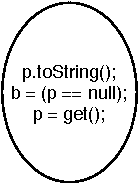
\includegraphics[]{figure/original-block-cfg.pdf}  &
		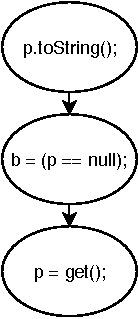
\includegraphics[]{figure/splitted-block-cfg.pdf}   \\ 
		Original block & Splitted block
	\end{tabular}
\end{figure}

Figure \ref{figure:new-way-to-split} shows the old and new control flow graph for the code of listing \ref{lst:native-block-creation}. 
By doing this, we will be able to support the example showed in listing \ref{lst:native-block-creation}, the check for \emph{null} breaks the block in three, the use and check will therefore not be in the same basic block.

Once the \emph{gen} (equation \eqref{eqn:dataflow3}) and \emph{kill} (equation \eqref{eqn:dataflow4}) set has been generated for every basic block, we can start to run the analysis with a work list approach.
The idea is to add all basic blocks in a queue and compute the new \emph{out} set of the current head. 
Since we are performing a forward analysis, if the new \emph{out} set have changed, this means that all the successors might potentially change as well. 
We add the current basic block and all of its successor at the end of the work-list, if the processed block sets have changed. 
We continue this process until the list is empty, meaning that we have reached a fixed point.

At the end of this process, we have a set of pointers believed to be not \emph{null} in each basic block.
We can therefore perform a second pass through the elements of the basic blocks, if we see a check for \emph{null} in a block where the pointer is in the set of believed to be not \emph{null}, we have a contradiction and we can report an issue.

\subsection{Other way to add belief}
\label{subsec:other_way_to_add_belief}

\emph{Null} pointer exception does not occur only when a \emph{null} pointer is dereferenced, but can also appear in the following cases for Java, as defined in the documentation \cite{OracleDoc:2019:Online}:

\begin{enumerate}
	\item Calling the instance method of a \emph{null} object;
	\item Accessing or modifying the field of a \emph{null} object;
	\item Taking the length of \emph{null} as if it were an array;
	\item Accessing or modifying the slots of \emph{null} as if it were an array;
	\item Throwing \emph{null} as if it were a \emph{Throwable} value.
\end{enumerate}
Currently, our checker is only using the first case, but we can use this information to improve our implementation: when we see one of these constructions, we will add the pointer to the set of believed to be \emph{non-null} (\emph{gen} set) the same way as we would for a pointer used.



\section{Implementation on SLang}
\label{sec:implementation_slang}

In the implementation on SonarJava, we had access to the front end of the checker, with complete tree, a control flow graph and the symbol resolution available.
The first step to implement it on \slang{} is to identify what nodes and structures we need in order to implement everything that is required for this check.

\subsection{Required Nodes}
\label{subsec:nodes}

The particularity of \slang{}  is that it is incomplete. 
The intermediate representation does not need to include all node types in order to work, only the one needed for the checks are mapped. 
We therefore have to make sure that we have all the nodes that we need in \slang{} for the implementation of the checker.

\begin{table}[h]
	\caption{Nodes needed for the null pointer dereference check}
	\label{table:nodes-needed}
	\begin{tabular}{|c|c|c|}
		\hline
		\bf Checker specific & \bf Needed for CFG & \bf Others  \\ \hline
	    Binary operation & If/else & Variable declaration \\
		Identifier & Switch & Function invocation \\
		Assignment & Exception handling, throw  & Function declaration \\
		Litteral : Null & Loops & Class declaration \\
		Member select & Jump (break, continue, …) & \\ \hline
	\end{tabular}
\end{table}

Table \ref{table:nodes-needed} shows the nodes that we need in order to implement the different parts of the checker.
The first column lists the nodes needed to recognize the different structures used in the checker. 
We can see that the list is quite simple. 
The interesting node is the member select, in fact, to identify when a pointer is used, we will only use this node: we do not need to know anything about the context in which the pointer is used, just that it is dereferenced at some point.
When a function is called without a member selection, the tree will be an identifier (name of the function) and a list of argument, but in the case of a pointer use, the tree corresponding to the identifier will be a member selection, that we will use in the checker.
By doing this, we can detect not only functions invocations, but also fields selections or anything that we consider as a member selection in the original language.

The nodes needed for the control flow graph are the one that we can expect for identifying the control flow of a program, that are mostly common in all language and already implemented in \slang{}. 
The way we handle them will be described in subsection \ref{subsec:cfg_on_slang}.
The last column describes other nodes that are needed indirectly by the checker:
\begin{enumerate}
	\captionsetup[lstlisting]{format=listingEnum, labelfont=white, textfont=white, singlelinecheck=false, margin=0pt, font={bf,footnotesize} }
	\item \textbf{\textit{Variable declaration}} \newline
	\lstinputlisting[label={lst:local-scope-in-while},
	caption=Local scope inside a loop that can shadow a field]{code/local-scope-in-while.scala}
	
	In section \ref{subsubsec:identifying_local_variable}, we are going to describe how we perform a naive semantic, that is assumed inside the check.
	In this semantic, we are not going to be able to differentiate if two pointers that have the same name refer to the same declaration.
	The idea to better support this limitation is that we will kill the pointer in the analysis when we see a declaration, the same way we are killing it when we see an assignment.
	In listing \ref{lst:local-scope-in-while} the pointer is used at line $\#1$ and check for \emph{null} at line $\#4$, but the two identifier \emph{p} do not refer to the same symbol.
	In this case, removing \emph{p} from the set when it is declared at line $\#3$ will enable us to remove the false positive.

	\item \textbf{\textit{Function invocation}} \newline
	\lstinputlisting[label={lst:function-invocation-support},
	caption=Pointer used as a parameter of a function call]{code/function-invocation-support.scala}
	
	As discussed before, we do not need explicitly function invocation, only member selection. 
	Due to a specific way we handle nodes that are not translated that we will explain in section \ref{subsec:how_to_deal_with_native}, we will add function invocation to be able to report pointer use that happens inside a function call, as illustrated in listing \ref{lst:function-invocation-support}.
	
	\item \textbf{\textit{Function and Class declaration}} \newline
	As our checker is only ran inside functions, we need function declaration to have our starting point. 
	We also use this to improve our semantics, using the fact that the variable that is used inside a nested function is not checked.
	
	Class declaration is used for the same idea as the function declaration, we use the assumption that variable declared in nested class are in another scope.
\end{enumerate}

\subsubsection{Other nodes not supported}
\label{subsubsec:other_nodes_not_supported}

In \ref{subsec:other_way_to_add_belief}, we saw multiple way to add the belief that a \emph{null} pointer can be raised. 
Slang do not have arrays, so we could expect to not find all issues coming from them. 
The first is the length of the array, in Slang, this is represented as a member select, and can therefore be supported.
Accessing or modifying the fields of \emph{null} as if it were an array is however not supported. 
This will lead to false negatives in \slang{} that we will not have in the implementation of SonarJava, but the situation seems to be uncommon.

\subsection{Control Flow Graph on SLang}
\label{subsec:cfg_on_slang}

\slang{} already have every control flow statements represented in the language, we can already start to build it the same way we would do it for any other language. 
In fact, the current implementation is greatly inspired by the one of SonarPHP \cite{SonarPHP:2019:Online}, also developed at SonarSource.
To build the control flow graph, we are going to use two main kind of basic blocks:

\begin{enumerate}
	\item \textbf{\textit{CFG Block}} \newline 
	This is the base of all basic block of the graph, it contains 4 fields:
	\begin{enumerate}
		\item \textbf{\textit{Predecessors}} \newline
		List of nodes that may be executed \textbf{before} the current block.\newline
		\item \textbf{\textit{Successors}} \newline
		List of nodes that may be executed \textbf{after} the current block.\newline
		\item \textbf{\textit{Elements}} \newline
		List of instruction that are executed one after the other in this basic block. \newline
		\item \textbf{\textit{Syntactic Successor}} \newline
		List of node following the current block if no jump is applied. 
		This is not directly needed for our check, but it may be required for some check later in the future.\newline
	\end{enumerate}
	\item \textbf{\textit{CFG Branching Block}} \newline 
	This interface represents blocks that include branching instruction, where the flow depend on the result of a Boolean expression. 
	It inherits from CFG Block and have a true and false successor block reference in addition to the simple block.
	\newline 
\end{enumerate}
This is the only two interface that we need, we can now start to build the graph.

\subsubsection{Building the control flow graph}
\label{subsubsec:building_the_graph}
Since we are going to build a graph for the content of a function, our starting point will be the list of the elements of the function.
We are going to start from the end of the execution, using a bottom-up approach.
It enables us to always know the successor of the node that we are currently building, making easier to build the different instructions that contain control flow.
We start by creating an \emph{END} node, that contains no element and represents the end of the execution.
We will then recursively build the graph by matching on the type of the tree.

\begin{enumerate}
	\captionsetup[lstlisting]{format=listingEnum, labelfont=white, textfont=white, singlelinecheck=false, margin=0pt, font={bf,footnotesize} }
	\item \textbf{\textit{Block and other nodes}} \newline 
	\label{subsubsec:block_and_others}
	The simplest tree that we will face are the blocks, they represent a list of statements, we can therefore directly recursively build the graph for all children, that will add the content of the block inside the current basic block. 
	This behavior can also be applied to other known trees that does not change the flow of execution, as a default case.
	The only difference is that we are also going to add the current tree to the elements after having built the graph for the children, in order to keep useful information. 
	For example, having a list of identifiers is not useful if we do not know that they are linked together by a binary expression, we will therefore add both the binary expression and the children to the elements of the current block.
	
	\item \textbf{\textit{If/Then/Else}} \newline 
	\label{subsubsec:if_then_else}
	This is the typical example that implements a branching block. 
	We will first build the sub flow for the false and true branch, if present, and then construct a branching block with these two new blocks as false and true successors, respectively.
	We can now recursively build the condition of the \emph{If} tree from the branching block created before.
	
	\item \textbf{\textit{Loops: For, While, Do-While}} \newline 
	\label{subsubsec:loops_cfg}
	The bottom-up approach makes the creation of the \emph{If} tree straightforward, since we have already built the successor of the tree that we are currently building. 
	However, in the case of loops, the flow is not going to continue at the successor, but return at the condition of the loop, a predecessor’s node that we have not built yet. 
	To address this situation, we can introduce a \textbf{forwarding block}, a basic block that is used to store a reference and will not contain any element.
	We can now start to build the loop flow by creating a forwarding block that will link to the condition and build the body with this new block as the successor. 
	Finally, we can build the condition of the loop as a branching block, with the true successor as the body of the loop, and the false as the block that follow the loop.
	There is one details that we have not address yet: break and continue.
	To support these two statements, we are going to use a stack, that will contain \textbf{breakable} objects. 
	These temporary objects are here to store the link to the condition for emph{continue}, and the end of the loop for \emph{break}.
	Before starting to build the body of the loop, we will push a breakable object to the top of the stack, and pop it once we are done. 
	We use a stack to support nested loop, a break and continue will refers to the first enclosing loop.
	
	The current implementation of \emph{For} loops is the same as \emph{While} loops, as we do not need the exact behavior of loop for our check, we can accept this approximation.
	For \emph{Do/While} loops, we are going to use the same idea but we are going to start to build the condition before the body.
	
	\item \textbf{\textit{Match Tree}} \newline 
	\label{subsubsec:match_tree_cfg}
	The particularity of a match tree is that it can behave differently depending on the original language.
	For example, in Scala, only one match case can be executed, while in Java, all cases are executed after a matching pattern, until a \emph{break} statement.
	The second example is typically known as fallthrough. 
	In \slang{}, both of them are mapped to the same node, however, identifying which one is the right behavior can be done by storing a flag in the node.
	Non-fallthrough match tree is an easy case, we can build all the cases separately, and create a block that will have multiples successors.
	
	Fallthrough switch is trickier, we first have to use the same idea as we used for loops: add an object (similar to breakable), to the stack, to store the reference to the block that is executed after the switch. 
	We make the same assumption as we did with loop, that a \emph{break} statements refer only to the closest enclosing match tree. 
	
	The next step is to create a forwarding block for the default case of the match tree, and build the different cases in the reverse order, one after the other. 
	We create one branching block per match cases, with the body of the case as true successor and the next pattern as the false successor. 
	At the same time, we can build the sequence of the body of cases, re-starting each time we see a break.
	
	\lstinputlisting[label={lst:pattern-match},
	caption=Fallthrough pattern matching]{code/pattern-match.scala}
	
	\begin{figure}[h]
		\caption{Listing \ref{lst:pattern-match}'s corresponding CFG }
		\label{figure:pat-mat-cfg}
		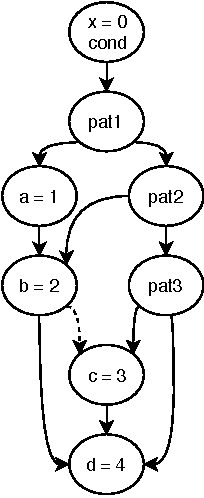
\includegraphics[]{figure/pat-mat-cfg.pdf}
	\end{figure}
	
	Figure \ref{figure:pat-mat-cfg} shows the resulting control flow graph of the code of listing \ref{lst:pattern-match}. We can see that the fallthrough behavior is represented as expected, for example \emph{a = 1} is executed both when \emph{pat1} and \emph{pat2} is true.
	
	\item \textbf{\textit{Jump Tree: break and continue}} \newline 
	\label{subsubsec:jump_tree_cfg}
	
	Jump trees are not supposed to appear when we do not expect them, if we have an unexpected jump tree, we cannot do anything, and we will directly add it to the current block. 
	We will discuss in section \ref{subsec:how_to_deal_with_native} a solution to better support this situation.
	In the usual case, they will appear where we expect them and create an edge from the current block to the head of the stack that is filled as described in \ref{subsubsec:loops_cfg} and \ref{subsubsec:match_tree_cfg} sections.
	
	\item \textbf{\textit{Return}} \newline 
	\label{subsubsec:return_cfg}
	Once again, starting from the end greatly simplify the support of return statements: we can store a reference to the \emph{END} block that is created at the beginning, use it as successor to the block that will contain the return expression.
	
	\item \textbf{\textit{Exception Handling Tree and Throw Tree}} \newline 
	\label{subsubsec:exception_handling_cfg}
	In our control flow graph, we are only going to consider exception that are explicitly thrown with a throw statements, and not add an edge to every statement where an exception can occur in reality. \newline
	We are going to start at the end of the exception handling tree. 
	When an exception handling tree is executed, it can result in two possible cases: the exception is caught and the flow can continue, or it is not and the flow goes to the end of the function. 
	To support this behavior, we are going to create a block with two successor: the \emph{END} node and the successor previously created. \newline
	We can then create the \emph{finally} block, if present, and the different catch case separately, and continue to build the body of the \emph{try} block. 
	At this point we must know where to jump in the case where an exception is thrown. 
	To do this, we will use the same idea as we did with the jump trees: use a stack to push the target of the throw before building the body, and popping it after. 
	If there is no catch block, the target will be the \emph{finally} block, if there is one or more catch block, we will use the first catch case as target. 
	This is an approximation that is due to the fact that we have no symbol resolution, we cannot know which and where the exception is caught.
	From now, we can know where to jump in the case of a throw three.\newline
	The last detail to take care of is the case where we have a return inside an exception handling tree.
	In this case, the \emph{finally} block is executed after the return. 
	To support this, we will store the exit target on a stack, pushing the reference to the finally block on top of the \emph{END} block previously added.
	
	\item \textbf{\textit{Natives Nodes}} \newline 
	\label{subsubsec:native_nodes_cfg}
	The main challenge comes from the only new nodes that we have compared to any language: the \emph{natives nodes}. 
	The way we deal with native nodes will be described in subsection \ref{subsec:how_to_deal_with_native}.
\end{enumerate}

\subsubsection{Normalization}
\label{subsubsec:normalization_cfg}
The core of the graph is done, but we still need to perform a few modifications in order to have a proper control flow graph. 
First, we are going to remove empty blocks. 
They can be introduced in multiple situations, when we create a temporary forwarding block or when the header of a \emph{For} loop is empty for example.
During the creation of the graph, we only knew the successors of the nodes, we still have to compute the predecessor set. 
Since we have all successors, the task is straightforward. 
Finally, we can create a \emph{START} node, that implements the same behavior as the \emph{END} node, to indicate the beginning of the flow. \newline
The hard work is done, we now have a complete control flow graph. 
There is still part of it that can be imprecise due to the fact that the different statements of the original language can behave differently, but we are going to discuss it later in section \ref{subsec:how_to_deal_with_native}.

\subsection{Data flow analysis}
\label{subsec:data_flow_analysis}

We now have all nodes needed and a control flow graph, we can start the implementation of the checker, that is in fact really similar to the one described in \ref{sec:implementation_java}. 
The main difference is the way we deal with nodes that have an unreliable execution order and the identification of local variable.
The former will be described in \ref{subsec:how_to_deal_with_native} and the latter in the next section.

\subsubsection{Identifying local variable}
\label{subsubsec:identifying_local_variable}

In SonarJava, we have access to symbol of identifier, data that we do not have in \slang{}. 
The current computation of local variable is quite simple: all variable declaration inside the function and all arguments are considered as local variables.
This is a naive version that is not made to work well for all language but used to show that with a proper semantic computation (name definitions and scoping rules) we could expect results that are as good as the current naive version. \newline
When we have this set of local variables, we can now check if the variable is in this set before reporting the issues. 
In practice, we could still report the issues that are not coming from local variable, but this would add some false positive.

\lstinputlisting[label={lst:field-change-value},
caption=Field can change value during a function call]{code/field-change-value.scala}

Listing \ref{lst:field-change-value} shows an example of a false positive due to a function with side-effect that change the value of a field. 
Adding the issues that come from non-local variable double the number of issues found, but the most of them are false positives.
Since a variable can be reassigned between the use and the check of a pointer, these new issues do not exactly respect the original description, we are not going to report them.

\subsection{How to deal with native nodes in a CFG based checker?}
\label{subsec:how_to_deal_with_native}

It is finally time to explain how we are going to deal with the native nodes.
For our concern, we will see the native nodes as a node that we do not know anything about, with a list of children.

\lstinputlisting[label={lst:ternary-expression-belief},
caption=Simple ternary expression]{code/ternary-expression-belief.scala}

\begin{figure}[h]
	\caption{\slang{} AST from the code of listing \ref{lst:ternary-expression-belief}}
	\label{figure:ternary-ast}
			\Tree[.... 
				[.\color{red}Native
				[
					\textit{true}
					\textit{b}
					\textit{p.toString()}
				]
				]
				\textit{p == null}
				]
\end{figure}
Figure \ref{figure:ternary-ast} shows the result of the \slang{} tree created from the code from listing \ref{lst:ternary-expression-belief}. 
In this example, we assume that we do not have ternary expression in \slang{}, and that they are not mapped to \emph{If/Then/Else} statement. 
We will use ternary expression of Java to represent the problem, but the construction can be any native nodes coming from any original language. \newline
The problem here is that we must represent the control flow of a node that we do not know anything about.
We cannot trust the evaluation order of the children of the native nodes, as it can be arbitrary. 
The first question that arise is why do we have to keep the content of a node that we do not know anything about? In fact, this is the root of the idea of the native nodes, we are not interested in the node itself, but only on the content.

\begin{figure}[h]
	\caption{CFG with an assignment in a native node}
	\label{figure:cfg-with-assignment-native}
	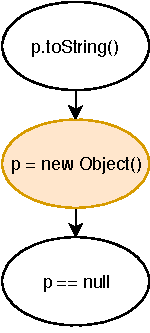
\includegraphics[]{figure/cfg-with-assignment-native.pdf}
\end{figure}

Figure \ref{figure:cfg-with-assignment-native} shows a typical example: in this case, we do not need to know what the native node (orange node) is exactly, but that the node assign \emph{p}. We do not care what exactly happens in this native node, we just need to know that, at one point, \emph{p} is assigned, even if it is possible that the assignment is never executed. If it is the case, this will add false negative, but intuitively, we can assume that dead code is not common, and this will not happen very often.

So, at this point, we know that we need to keep the content of the native nodes. 
The next step is to define what to do with them. 
A naive solution would be to add the content of the graph in the elements of the basic block, assuming that the evaluation order is not important. 
This is in fact correct for a native node with only one child, where the evaluation order can obviously not change. 
If there is multiple children, we have to add the assumption that all the statements that change the flow of a program are represented in \slang{}. 
This is a reasonable assumption since programming language hardly ever provide exceptional statement that are break the control flow, and if it does, we can add it to \slang{} grammar.

\lstinputlisting[label={lst:ternary-expression-example},
caption=Pseudo code with a ternary expression]{code/ternary-expression-example.scala}

\begin{figure}[h]
	\caption{Basic block content of the code in listing \ref{lst:ternary-expression-example}}
	\label{figure:basic-block-content}
	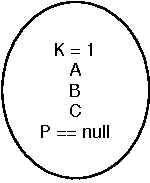
\includegraphics[]{figure/basic-block-content.pdf}
\end{figure}


Listing \ref{lst:ternary-expression-example} some Java pseudo code with the corresponding control flow graph with the naive implementation in figure \ref{figure:basic-block-content}.
Since the ternary expression will be mapped to a native node in \slang{}, if we take the children of the native node in order, we will obtain the execution order of the nodes in figure \ref{figure:basic-block-content}, that is obviously not correct, as the pointer will be seen as used then checked in this order, but it is not in the real execution.

\begin{figure}[h]
	\caption{CFG with elements coming from natives nodes}
	\label{figure:two-unreliable-cfg}
	\setlength{\tabcolsep}{24pt}
	\begin{tabular}{cc}
		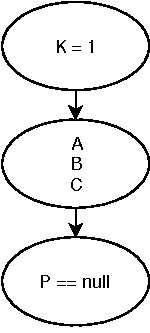
\includegraphics[]{figure/unreliable-cfg-1.pdf}  &
		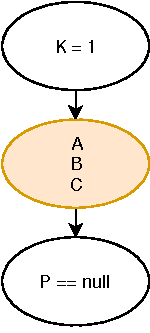
\includegraphics[]{figure/unreliable-cfg-2.pdf}   \\ 
		Split CFG & Split block with unreliable node
	\end{tabular}
\end{figure}

We can therefore not ignore these nodes, and not naively add them to the blocks.
The idea to solve the problem showed before is to put all elements that come from a native node in a separate basic block (figure \ref{figure:two-unreliable-cfg}, left), and mark the block as \textbf{unreliable} (figure \ref{figure:two-unreliable-cfg}, right), shown in orange.
All control flow statement nested inside the native nodes will also lead to unreliable basic block.\newline
Additionally, we will also mark the whole graph as unreliable. 

This information can now be used by any checker that use a control flow graph, not only for the \emph{null} pointer dereference checker.

\subparagraph{How to use this information?}
\label{subsubsec:use_unreliable_information}

This information can be used in different ways to help to define the multiple level of granularity of the implementation of a new checker:

\begin{enumerate}
\captionsetup[lstlisting]{format=listingEnum, labelfont=white, textfont=white, singlelinecheck=false, margin=0pt, font={bf,footnotesize} }
\item \textbf{\textit{Ignore this information}} \newline
In some case, it may make sense to ignore this information, and to treat unreliable nodes as others. 
In our case, we have shown previously that this solution is not suitable, as it produces too many false positives. \newline

\item \textbf{\textit{Don’t run the checker on unreliable CFG}} \newline
This is the opposite of the previous point: in the case where the checker needs to really trust the control flow graph, it can make sense to directly stop the checker if the graph cannot be trusted.

\begin{table}[h]
	\centering
	\caption{Percentage of native and completely native nodes in the different languages}
	\label{table:slang-native-percentage}
	\begin{tabular}{|c|c|c|c|}
		\hline
		\bf Language & \bf \% & \bf \% of completely native & \bf $\bf N^{\circ}$  of files \\ \hline
		Scala &  41 &  6.25 & 6126 \\ 
		Kotlin &  47 &  6.5 & 26758 \\ 
		Ruby &  39 &  5.2 &  7811 \\ \hline
	\end{tabular}
\end{table}

Table \ref{table:slang-native-percentage} show the percentage of native nodes in \slang{} after translating open-source projects \cite{SlangSources:2019:Online} to \slang{}. The percentage of completely native nodes refers to the nodes that have all their children as native. If more than $40\%$ of nodes are not translated, this does not mean that our language lack a lot of nodes, but that we do not mapped some kind of nodes on purpose.
This table shows us that native nodes are not rare, using the above approach will greatly reduce our chance to find any relevant issue as we will, in the most of the case, be in the presence of native nodes in the body of a function.

The two approaches described before seems not well-suited for our checker, we may want something between the two extremes.

\item \textbf{\textit{Fine grain}} \newline
We can use the fact that we know if an element comes from a native node or not to define a finer grain implementation of our checker. 
It consists mainly in one modification of the data flow analysis described previously: we do not add a pointer that is used in an unreliable block to the believed to be \emph{non-null} set.

\begin{equation}\label{eqn:new_dataflow4}
newGen(n) = \parbox{7cm}{use of pointer in the node n, \newline except if the node is marked as unreliable}
\end{equation}

\lstinputlisting[label={lst:fine-grain-1},
caption=First example of finer grain behavior]{code/fine-grain-1.scala}

\lstinputlisting[label={lst:fine-grain-2},
caption=Second example of finer grain behavior]{code/fine-grain-2.scala}

With this idea, we are now avoiding to report any issue for the two correct pseudo code from listing \ref{lst:fine-grain-1} and \ref{lst:fine-grain-2}. Since ternary expression are unreliable, we will not consider \emph{p} as used, even though it may look like in the control flow graph.

\lstinputlisting[label={lst:fine-grain-3},
caption=Third example of finer grain behavior]{code/fine-grain-3.scala}

In listing \ref{lst:fine-grain-3} though, the real evaluation order use \emph{p} and then check it for \emph{null}. 
This code is not reported by our tool despite the fact that it should be. This is a false negative.\newline

\lstinputlisting[label={lst:fine-grain-4},
caption=Fourth example of finer grain behavior]{code/fine-grain-4.scala}

In addition, the implementation will still report issues inside native nodes.
For example, in listing \ref{lst:fine-grain-4}, we can see that the pointer \emph{p} is used, and then checked for \emph{null} later in a un-trusted node. We do not know exactly what exactly happen in this node, but we can expect that a check for \emph{null} still mean that p can be \emph{null}. 
In this example, we report an issue, that is a true positive.
\end{enumerate}

\subsection{Other problematic situations}
\label{subsec:other_problematic_situation}
	
We have already presented the main problematic situations, coming from native nodes, but there are still a few cases that can raise false positive that we have to take care.

\begin{enumerate}
	\captionsetup[lstlisting]{format=listingEnum, labelfont=white, textfont=white, singlelinecheck=false, margin=0pt, font={bf,footnotesize} }
	\item \textbf{\textit{Boolean short-circuit}} \newline 
	\label{subsubsec:boolean_short_circuit}
	Our current implementation of the control flow graph does not encode the possible path due to Boolean short-circuit. 
	This will lead to a wrong evaluation order, even if the nodes are known. 
	Since the evaluation order is not correct, it makes sense to treat them the same way we do with native nodes! 
	We will hence keep all the content of these nodes, to be able to use them in the checkers, but mark them as unreliable. 

\lstinputlisting[label={lst:boolean-short-circuit},
	caption=Problematic situations due to Boolean short circuit]{code/boolean-short-circuit.scala}
	
	With this addition, we are now able to avoid the false negative that were reported in the two examples of listing \ref{lst:boolean-short-circuit}.
	
	\item \textbf{\textit{Order of evaluation of known nodes}} \newline 
	\label{subsubsec:evaluation_known_nodes}
	In section \ref{subsec:how_to_deal_with_native}, we have seen that the order of evaluation of the nodes are critical for our checker.
	When coming from different languages, even known nodes can have different evaluation order, as we have seen an example in section \ref{subsubsec:match_tree_cfg}. 
	The same situation can in fact arise for any statement, hopefully, the solution is often to add the support for the new behavior in \slang{}.
	This trick should be used with caution, the initial goal is to be language agnostic, we should ideally not have to modify \slang{} for every new language we add. 
	The good news is that there is only a limited number of variations that are possible, since the number of known nodes is fixed (and only a fraction of it in practice). 
	This kind of problem are difficulty that are hard to anticipate and will arise during the implementation of a new checker, but it is not in itself a strong limitation.
	
	\item \textbf{\textit{Lost Jump Statements}} \newline 
	\label{subsubsec:lost_jump_statement}
	We have seen in section \ref{subsubsec:jump_tree_cfg} that we directly a jump statement to the basic block in the case where we do not expect it, without doing anything special.
	In fact, we face similar uncertainties that happen with native nodes, we do not know exactly what is happening, but we can expect that something will go wrong.
	The same happen with jump tree with label, as the way the different language deals with label can be arbitrary, we cannot assume anything.
	We just know that the statement will change the execution flow in an unreliable way, we will therefore mark the flow generated by this statement as \emph{unreliable}.
\end{enumerate}

\section{Running the checker on open source Java projects}
\label{sec:running_checker}

In this section, we are going to compare the implementation of the checker on \slang (\ref{sec:implementation_slang}) with the implementation on SonarJava (\ref{sec:implementation_java}), on a set of open source Java projects. It is a good source of data since it enables us to test the result on real situation.

\subsection{Experimental Setup}
\label{subsec:experimental_setup}

To test the checker, we are going to create a SonarQube instance \cite{SonarQube:2019:Online}, with the version of the checker that we want to test. We are going to run the analysis with the plugin containing the implementation of our checker on more than 100 open source projects and publish the results on the SonarQube instance. Table \ref{table:issues-per-project} shows a sample of the projects list, and the complete list can be found in Appendix \ref{app:open_source_projects}.

\subsection{Early results}
\label{subsec:early_results}

The checker has been run on more than one hundred of project of various size, containing for instance OpenJDK, SonarJava and the \slang project itself. 
The idea is to run the implementation done on SonarJava and \slang, and compare the results.

\begin{table}[h]
	\centering
	\caption{Early number of Issues reported by the two implementation, before improvement}
	\label{table:early-sonarjava-vs-slang}
	\begin{tabular}{|c|c|c|}
		\hline
		\bf SonarJava issues & \bf Slang issues & \bf \% \\ \hline
		37 &  29 &  78 \\ \hline
	\end{tabular}
\end{table}



Table \ref{table:early-sonarjava-vs-slang} shows the number of issues reported by the implementation on SonarJava, and the issues reported by the implementation on \slang, with the source, setup described in section \ref{subsec:experimental_setup}. 
Despite all our effort to prevent problematic situation done in the previous parts,  the implementation is having more than 20\% of false negative compared to the implementation on SonarJava. This is already a good start, but it is not enough for our objective set in section \ref{subsubsec:precision_recall}.
We can wonder what are the reasons of this differences.
We will discuss some of them in the following part, to see if this comes from a misbehavior of the implementation, or a real limitation of \slang.

\subsection{Reducing the false negative from SonarJava}
\label{subsec:reducing_false_positive_sonarjava}

The difference between the two implementations is mainly due to the way ternary expression and loop header is currently handled in \slang.

\subsection{Ternary expression}
\label{subsec:reducing_false_positive_ternary}
Ternary expression have been used as example previously, and they actually appear to be causing false positive in real project.

\lstinputlisting[label={lst:reduce-fp-ternary},
caption=Typical code structure with ternary expression]{code/reduce-fp-ternary.scala}

The situation is not as obvious as the one presented before, listing \ref{lst:reduce-fp-ternary} show a possible situation were no issues will be reported. To solve this problem, one solution is to map ternary expression to if/else tree.This solution is already used for other checks and seems to solve our problem nicely.

\subsection{Loop Header}
\label{subsec:loop_header}

Currently, no rules uses the details of the for loop header, it is therefore mapped to a native tree. 

\lstinputlisting[label={lst:loop-header},
caption=Pointer used inside loop header]{code/loop-header.scala}

Listing \ref{lst:loop-header} shows the problematic situation. The pointer \emph{p} is used, not re-assigned, and check for null later. 
It is exactly the kind of situation that we would like to report. 
However, the different parts of the header are in a native node, as described before, it will therefore not be added to the set of used pointer. 
This makes sense, from a language agnostic point of view, we can not know anything from the execution order of the different block of the loop header, as it can depends on the original language for example. 
This is in fact the kind of behavior that we want to achieve, the language specific features does not produce false positive, we only have false positive. 
One way to solve this problem is to simply add a node in \slang that will better support this situation. 
If it makes sense for loop header as it is probably a feature that is present in different situation, we have to keep in mind that this is not a solution that we should use in all situation, where the feature is really specific to a language.

\subsection{Improved results}
\label{subsec:improved_results}

\begin{table}[h]
	\centering
	\caption{Final issues found by the two implementations for Java}
	\label{table:final-sonarjava-vs-slang}
	\begin{tabular}{|c|c|c|}
		\hline
		\bf SonarJava issues & \bf Slang issues & \bf \% \\ \hline
		37 &  37 &  100 \\ \hline
	\end{tabular}
\end{table}

With the two modification done on the implementation on \slang, , with the same source and setup described in section \ref{subsec:experimental_setup}, we manage to report the same issues that the implementation of SonarJava was reporting!

\begin{table}[h]
	\centering
	\caption{Final issues found by the two implementations for Java, with the source and setup described in section \ref{subsec:experimental_setup}}
	\label{table:issues-per-project}
	\begin{tabular}{|c|c|}
		\hline
		\bf Project & \bf Number of issues\\ \hline
		OpenJDK 9 & 12 \\
		ElasticSearch & 7 \\
		Apache Abdera & 5 \\
		Apache Tika & 	4 \\
		Ops4j Pax Logging & 3 \\
		Apache Jackrabbit & 2 \\
		RestComm Sip Servlets & 1 \\
		Wildfly Application Server & 1 \\
		Apache pluto & 1 \\
		Fabric8 Maven Plugin & 1 \\\hline
		Total &  37 \\ \hline
	\end{tabular}
\end{table}


Table \ref{table:issues-per-project} shows the projects that contains one or more issues and number of true positive reported, for both forward and backward analysis. All these issues have been reported by both the SonarJava implementation, and Slang with the modification done in Reducing the false negative from sonarJava.


\subsubsection{Other languages}
\label{subsubsec:other_languages}

The mapping to \slang has been implemented for 5 languages: Java, Scala, Kotlin, Ruby, and Apex. Once we have an implementation of a checker that works for one language, the checker can be run out of the box on other languages if we make sure that all node described in subsection \ref{subsec:nodes} are present.

[TODO: run on 1000s] \newline

[[ The checker seems to work on some sample example, but does not manage to find any real issues on the project that we tested. For Apex, this can be explained by the fact that we have only little open source code available out here. For Scala and Kotlin, the two languages provide a special construct to deal with null. Therefore, we can expect less issues on these two language. Comparing the performance of the checker for Scala and Kotlin with other tool is not really possible, since the only check that exists and make sense in these language is simply that you should never use Null.]]

\subsection{Are the issues found really relevant?}
\label{subsec:are_the_issues_relevant}

Table \ref{table:issues-per-project} shows the number of issues found per project. 
This includes all the true positives of the forward and backward analysis. 
A first observation is that the issues found are coming from various project and in various situations, it is not one anti-pattern that is repeated multiple times in the same project. Additionally, all the issues seems to be relevant from a high level view and without any specific knowledge of the project, you can not easily justify any of the issues reported. 
To estimate more reliably this interest, we can also look at the fix rate of the issues.

\subsubsection{Fix-rate}
\label{subsubsec:fix_rate}

Fix-rate is the rate of issues that are reported by a tool, and really fixed by the user. 
As discussed in Precision and Recall tradeoff, static analysis tools have to deal with the fact that if we report too much issues, we take the risk of reporting irrelevant ones and the user will not pay attention to them. 
This is where fix-rate may be useful, it shows that the user did really care about the issue, and took some time to fix it. \newline
The problem is obviously that we can not define at a given instant this rate, we can only retroactively look at this number, depending therefore on the time we gives to the user to fix the issues.
The goal is not to reach a precise number, but to find examples of issues that are fixed, to improve our confidence in the quality of the results.\newline
The first way we will estimate the fix rate is by using some of our test project that are not updated for every version. 
In practice, there is only a few, the main one that we will use is the OpenJDK. 
The issues reported comes from version 9, that we will compare with the version 11.

\begin{table}[h]
	\centering
	\caption{OpenJDK 9 issues fixed in version 11}
	\label{table:openJDK_issues}
	\begin{tabular}{|c|c|c|}
		\hline
		\bf OpenJDK V.9  issues & \bf Issues fixed in V.11 & \bf \% \\ \hline
		12 &  3 &  25 \\ \hline
	\end{tabular}
\end{table}

Table above shows that 25\% of the issues found on OpenJDK 9 have been fixed in the version 11. This may seems like a low number, but it seems to be the kind of results we can expect from this kind of estimation. For example, a research from Jetbrains \cite{Bryksin:2018:DAK:3236454.3236457} report that 32\% of the issues reported by their tool were considered as useful (rated with high value) by the person that were confronted to the issues. 
We can explain this by the fact that developer have priorities, especially in such big open-source project, fixing a bug that is already here and is apparently not causing any trouble have low priorities, even if this is a legitimate issue. 
SonarSource often refers to this idea as the “Fix the leak” approach: it does not make sense to spend considerable effort to fix every bug already present in the code if you keep introducing new one on new code, the same way you would not start to mop the floor during a flooding without having fixed the origin. \newline

One other way to estimate the fix-rate is to look into the issues reported by the tool, understand them, eventually write a unit test that raise an exception, and report this issues to let the owner of the project decide if this issue is worth the attention.
One of the problem is that sometimes, it is indeed possible to write a unit test that target a specific function and throw a null pointer exception, but it will never happen in real execution due to the fact that the programmer have an implicit knowledge about his code, reducing his interest in fixing the code. 
For example, if a user only calls a function only when he finds a specific element in a list, he will assume that the list will never be null. 
These kind of issues should however not directly be classified as false positive, as it can also report dead code.

\subsubsection{Potential Null Pointer Exception or Dead code ?}
\label{subsubsec:dead_code}

\lstinputlisting[label={lst:contradiction-code},
caption=Example of contradicting code that lead to dead code]{code/contradiction-code.scala}

Despite the fact that we try to find null pointer exception, some of the issues found can be considered as dead code, as they can never raise an exception in practice. 
For example, in listing \ref{lst:contradiction-code}, we can see that this code will never raise an exception. 
It comes from the fact that we implies beliefs from the code that a programmer writes, if he writes himself contradicting statement, we will still report an issue. 
In the situation of listing above, the checker does not take in consideration the check for null as a path-sensitive tool would do. \newline
One similar situation is that sometimes, it is indeed possible to write a unit test that target a specific function and throw an exception, but it will never happen in real execution due to the fact that the programmer have an implicit knowledge about his code. 
For example, if a user only calls a function if he find a specific element in a list, he will assume that the list will never be null in this function, and therefore the check is simply dead code. 
This will however not degrade the quality of the results, this is still raising poor practice and poor code quality, since this will be dead code that can confuse the user.











\section{Related work}
\label{sec:related_work}

There is a lot of work about variations of null pointer consistency check available in the open-source world.
The most relevant and closely related work that uses an universal representation is the micro grammar approach \cite{Brown:2016:BSC:2954679.2872364} that we will discuss in subsection \ref{subsec:micro_grammar}.
In subsection \ref{subsec:other_tools}, we will present the different techniques that other popular tools use to perform null pointer dereference check.
None of them implements the checks on an universal language, but it is a good way to understand the technologies that they use to perform the checks, and anticipate the problems that can arise if we want to implements equivalent features on \slang{}.

\subsection{Micro grammar}
\label{subsec:micro_grammar}

How to Build Static Checking Systems Using Orders of Magnitude Less Code \cite{Brown:2016:BSC:2954679.2872364} is raising a similar concern that we tried to solve. 
They observed that the current situation makes it hard to target new languages due to the complexity of the current systems. 
The main idea is similar to \slang{}, they implemented a checker that is based on an incomplete grammar, that is called micro grammars.
With this approach, they managed to implement a checker that is order of magnitude smaller than typical systems.
The results that they obtain is encouraging, they manage to find hundreds of issues with an acceptable false positive rate, even some of them that were not reported by they previous work. 
The idea is similar to island parsing, where the grammar only describe some part of a language, without requirement to have the whole syntax.

\begin{table}[h]
	\centering
	\caption{Issues reported on OpenJDK 8b132 by the micro grammar approach}
	\label{table:micro_grammar_issues}
	\begin{tabular}{|c|c|c|}
		\hline
		\bf Issues & \bf False positives & \bf \% \\ \hline
		42 &  3 &  7 \\ \hline
	\end{tabular}
\end{table}

\begin{table}[h]
	\centering
	\caption{Issues reported on OpenJDK 8b132 by \slang{}}
	\label{table:slang_issues_jdk8}
	\begin{tabular}{|c|c|c|}
		\hline
		\bf Issues & \bf False positives & \bf \% \\ \hline
		28 &  0 &  0 \\ \hline
	\end{tabular}
\end{table}

Table \ref{table:micro_grammar_issues} and \ref{table:slang_issues_jdk8} are showing the number of issues reported by the micro grammar approach and \slang{} on OpenJDK 8b132.
By reporting no false positive on Java code, our implementation performs better than the micro grammar that reports an already very low rate.
However, our implementation reports less issues.
Unfortunately, the paper does not provide the list of issues reported to help us identify the one that we are missing.
One probable explanation is that we choose to only report the issues that come from local identifier (subsection \ref{subsubsec:identifying_local_variable}), this approach does not report any false positive, at the cost of few false negative.
Both results are more or less similar, and both works reach the conclusion that it is possible to find interesting issues with an universal approach.

\subsection{Technology used by other tools}
\label{subsec:other_tools_technology}

If the initial goal is not to find as many issues as any other tool, looking at the features they provide is a good way to know how to improve the current checker and to anticipate if it is possible to implement them on top of \slang{}.
None of them uses an universal language, we are not going to compare two implementation


\begin{table}[h]
	\centering
	\caption{Tools that detect \emph{null} pointer dereference}
	\label{table:tools_features}
	\begin{tabular}{|l|}
		\hline
		\bf Tools \\
		\hline
		SonarJava \cite{SonarJava:2019:Online} \\
		FindBugs \cite{Hovemeyer:2004:FBE:1052883.1052895} and SpotBugs \cite{spotBugs:2019:Online} \\
		Fbinfer \cite{fbInfer:2019:Online} \\
		ErrorProne \cite{errorProne:2019:Online} \\
		IntelliJ IDEA \cite{intelJIDEA:2019:Online} \\
		\hline    
	\end{tabular}
\end{table}

Table \ref{table:tools_features} shows the list of tools that detect \emph{null} pointer dereference, that we can use to compare and understand the different technologies that are currently used.
A first observation of these tools shows that they are globally using similar technology, with different level of efficiency.
Our tool is however implementing only a fraction of these technology, mainly due to the fact that we did not target them in the first place since we tried to not become too complex. 
The next parts will discuss the main features that are used by others tools, for what this technology is good for, and if we can implement it on \slang{}.

\subsubsection{Interprocedural}
\label{subsubsec:inter_procedrual}

Our current checker is only supporting intraprocedural analysis, going further is obviously a way to find more issue, since it would enable us to learn belief from arguments not only inside one function, but also outside it.
The main difficulty is to define which function is called at run time, if it is possible to do it for one language, having a consistent way to do it in a language agnostic way is a real challenge. 
One of the way is to compute the summary of every function, and to use this information during the intraprocedural analysis. 
For example, we can store for every function if it can return \emph{null}, then when the result of this function call is assigned to a variable, we can consider it the same way as if it was \emph{null}. 
This idea is used by SpotBugs and will be described in subsection \ref{subsec:spotbugs_specific}. 
There is multiple other ways to perform interprocedural analysis, that represents more precisely the execution flow, however the ideas are complex and will not be described in this work.

\subsubsection{Requires the build}
\label{subsubsec:require_build}

Requiring the build can be perceived as a disadvantage, since compiling code and calling it static analysis seems to be a contradiction.
Using the build provides however so much information that the popular tools seems to all have opted for it.
This can make sense when the checking for error is integrated to the build process, but this is a real handicap when we want to have interactive feedback in an IDE or a pull request analysis, and is not possible in a cloud computing scenario, when you do not have access to the binaries. 
The recent trend however is to avoid using the build due to the disadvantage stated before.

In the situation of \slang{}, we will obviously requiring to have access to the binaries of the original language does not make a lot of sense, since it will contradict everything that is already in place.
In addition, the goal of \slang{} is not to be a complete language, it is therefore far from being possible to compile this new code. 
This adds a new challenge that \slang{} will probably face in the future, but it brings enough benefits to make the effort worth it.

\subsubsection{Guided by annotation}
\label{subsubsec:guided_by_annotation}

We have seen in section \ref{subsubsec:inter_procedrual} that interprocedural analysis is difficult operation, to help to reduce the complexity of the analysis, we can use annotation to help the tool report possible problems. 
Annotation are typically used to declare that a function can return a \emph{null} value, or that a function should never be called with \emph{null} as argument.

\lstinputlisting[label={lst:annotated-code},
caption=Example of annotated code]{code/annotated-code.scala}

In listing \ref{lst:annotated-code} for example, the function \emph{f} is guaranteed to never return \emph{null}, and the callee can directly dereference the result of this function without further checking..
For the parameters, it enforces that \emph{f} can give \emph{null} as a first parameter, but not for the second one.\newline
They are multiple flavor on how to do it, depending on what we want, for example, Error Prone is using a trusting analysis, meaning that method parameters, field, and method return are assumed \nullable{} only if annotated so. 
If we see the problem the other way, we could alternatively ask to explicitly mark as \emph{non-null} an argument that should never be \emph{null}.\newline
Annotations seem to be the most popular way to detect \emph{null} pointer exception currently, especially for interactive tools, it enables to detect most of the exceptions with a small effort on the programmer side. 
It is often worth to make this effort, it is useful not only for the checker, but also helps during the development of the program.
The downside of this method is that it requires a consistent and coordinate use of annotation in a whole project, consistency that is hard to achieve, even more when we want to introduce it in an old project.

Annotation could be added on top of \slang{}, finding annotation that are relevant for any language is possible if they share the same concepts. 
For example, a \emph{non-null} annotation makes sense in any language that has the concept of \emph{null}. 
In other cases, this can be more tricky; for example, the annotation \emph{initializer}, used in the context of \emph{null} pointer exception, can not be used in an language agnostic way, since the initialization is not the same in any language.\newline
One solution to this is to provide a way to configure the tool. 
Using configurable check is always a danger for the user experience. For example, NullAway is providing more than 10 configuration flags, some of them being mandatory, all of them related to \emph{null} dereference. 
In the context of \slang{}, having so much configuration to do for every checks and every language simply does not scale at all.\newline
An interesting note is that annotation are principally used is to help to reduce the complexity of the analysis, however no annotation is required to detect all pointer if we have a perfect interprocedural analysis.

\subsubsection{Path sensitivity}
\label{subsubsec:path_sensitivity}

Currently, our tool is using flow sensitive analysis, meaning that we are only interested in the order in which the statements are executed.
In addition, path-sensitivity computes and keeps additional information, based on statements seen along the path and avoid infeasible path. 
For example, if a pointer is checked for \emph{null}, the tool will know that the pointer is equals to \emph{null} inside the true branch, it will therefore report if the pointer is used or given to a function that expect a \emph{non-null} value.
For our purpose, we could also learn the value of a given pointer with assignment for example.

\lstinputlisting[label={lst:simple-np},
caption=Simple example of null pointer exception]{code/simple-np.scala}

Listing \ref{lst:simple-np} shows a simple code that obviously raise an exception. Our checker is currently not able to detect it, since it does not try to know the current value of a pointer.
Path sensitive tools would be able to find this kind of issues.
In addition, we could also use the path sensitivity to improve the \emph{MAY} analysis introduce in subsection \ref{subsubsec:may_vs_must}, to remove the obvious false positives. 
The main challenge of this kind of analysis is to deal with the fact that the number of path grow exponentially, making it hard to scale. 
In the current situation, we do not have path-sensitivity in our checker, but we already have all the features required, implementing it with the same constraints as an implementation over a original language seem to be possible.

\subsection{Popular tools}
\label{subsec:other_tools_features}

The idea here is not to describe in depth the exact functioning of a particular tool, but to describe some of the features implemented by other tools that can be interesting for our purpose of anticipating the potential problems of an eventual implementation on \slang{}.

\subsubsection{IntellJ IDEA}
\label{subsubsec:intellj_idea}

IntellJ is an IDEA, this is a particularly interesting since it requires interactivity, a user wants to see the issues being raised while he writes code, without having to rebuild the whole project. 
This tool is also performing a \emph{null} pointer analysis using annotation. 
It warns when the user use a pointer that is \nullable{}, without checking it for \emph{null}. 
To detect that a pointer is checked for \emph{null}, it uses a pattern that is customizable. 
This will not work if the user is using custom methods to perform the null-check. 
In this case, the user can use a contract, that would for example say that this method fail if the argument is \emph{null}, or more simply configure the custom function that perform the \emph{null} check.\newline
Having configurable setting for a check in \slang{} is far from being ideal, even if the effort to configure one check seems to be minimal, if we have a configuration to do for every rule, this can quickly becomes a nightmare for the user. 
All our work that try to reduce the overall complexity would be pointless if we have a configuration for every checks.


\subsubsection{Error prone: Null away}
\label{subsubsec:error_prone}

\emph{Null} away is a tool built on top of error prone. 
To perform \emph{null} pointer consistency, the process first checks if the value dereferenced is obviously \emph{non-null} (annotated \emph{@Non-null}). 
If it is not the case, it performs a data-flow analysis to try to show the that the value is \emph{non-null}. 
The data-flow analysis is using existing \emph{null} check into the code, therefore, if a field is annotated as \nullable{} and is dereferenced, an error will be reported only if the value is not checked for \emph{null}. \newline
The key idea here is to perform the analysis in multiple steps of increasing complexity, skipping costly part, like the creation of the control flow graph, if it is possible.
Having multiple steps is a particularly good idea for \slang{}, not only for performance, but also for the quality of the results. 
If we can report an issue, or prevent a complex computation before facing the uncertainties due to \slang{}, it may prevent us to make bad decisions.

\subsubsection{SpotBugs}
\label{subsec:spotbugs_specific}

We have seen in subsection \ref{subsec:indpeth_comparison_spotbugs} that SpotBugs is reporting way more issues related to null dereference that our implementation is reporting.
The main reason of this huge difference is in fact due to the features described previously in subsection \ref{subsec:other_tools_technology}.
In addition, we will look more in-depth into one additional feature that is implemented in SpotBugs and producing a big difference, and see if it may be implemented on \slang{}.

\begin{enumerate}
	\captionsetup[lstlisting]{format=listingEnum, labelfont=white, textfont=white, singlelinecheck=false, margin=0pt, font={bf,footnotesize} }
	\item \textit{Summary-based interprocedural analysis} \newline
	This is an smart and easy first step to perform interprocedural analysis.
	The idea is to compute a summary of every methods, and use this information during the intraprocedural analysis. 
	In our case, we would like for example to store if a method can return \emph{null}, or if a parameter could be \emph{non-null} to then report if \emph{null} is passed as his argument. 
	We can have this information by looking at annotation.
	If the annotation are not present, we can still perform intraprocedural analysis to infer ourselves the annotation. 
	For example, if a method ever return \emph{null}, we can annotate the function as \nullable{}, and if a function always dereference an argument without checking it for \emph{null}, we can consider the argument as \emph{non-null}. 
	The good part is that we already have the nodes and data required to build the summary. 
	The feature currently missing in \slang{} is the method reference. 
	We obviously need to be able to identify which method is called to be able to retrieve the summary.
	This is related to the problem of the name reference that we faced during in the previous parts, naive solution exist, but proper semantics have to be completed to obtain interesting results.
	
	
	\begin{figure}[h]
		\centering
		\caption{Pseudo code of a class that extends an abstract class}
		\label{figure:class-extends-abtract}
		\setlength{\tabcolsep}{24pt}
		\begin{tabular}{cc}
			\multicolumn{1}{c}{\lstinputlisting[numbers=none,nolol=true]{code/abstract-class-1.scala}} & \multicolumn{1}{c}{\lstinputlisting[numbers=none,nolol=true]{code/abstract-class-2.scala}} \\
		\end{tabular}
	\end{figure}
	
	\lstinputlisting[label={lst:spotbugs-true-false-positive},
	caption=Example of true and false negative of SpotBugs]{code/spotbugs-true-false-positive.scala}
	
	In listing \ref{lst:spotbugs-true-false-positive}, we have an example of a true positive and a false negative from SpotBugs. At line $\#2$, the issues is correctly reported, the tool manages to identify statically that the pointer \emph{b} is called with type \emph{B}. At line $\#4$ however, the tool is not reporting any issue. This is due to the fact that the type of \emph{a} is \emph{B}, the tool is not able to identify the potential run-time type of the variable.\newline
	Obtaining equivalents results does not require complex features, there is no strong push-back to implement it on \slang{}, and could already greatly increase the number of issues reported by \slang{}!
\end{enumerate}
\section{Future work}
\label{sec:future_work}

\subsection{Rule inference}
\label{subsec:rule_inference}

This work shows the potential of \slang{} to support the implementation of more and more checks, however, the list is limited, finding interesting rules that make sense in a language agnostic way is difficult. 
One promising continuation is to work on rule inference to detect object usage anomalies \cite{Wasylkowski:2007:DOU:1287624.1287632}. \newline
Rules inference tries to solve the problem that programmers use a wide range of functions for the same goal, identifying which function does what is typically a cumbersome process that needs to be done by hand and even impossible for manual approach if the function is user-defined. 
If the basic idea is to generate rules specific to a project, it would make sense to adapt it to generate rules specific to a language, everything in an agnostic way on top of \slang{}. 
The typical example is to look at temporal properties. 
There is multiples way to do it, looking at the sequence of method call during an execution \cite{Gabel:2010:OIE:1806799.1806806}, or to use an idea related to the belief style \cite{Engler:2001:BDB:502059.502041} that we used in this project. 
The idea is to learn pattern of sequence of function call from the code and report when this pattern is not respected.
For example, if we see that the majority of the time, \emph{$<b>$} is used after \emph{$<a>$}, it might imply the belief that \emph{$<b>$} should be called after \emph{$<a>$}. If, in the minority of the cases, \emph{$<b>$} is not called after \emph{$<a>$}, it contradicts the belief and may therefore imply an error. 
Concretely, this idea should be able to detect that an unlock is called after a lock, or that a resource is closed. 
In this example, the way a programmer typically deals with them is dependent on the language and even dependent on the project! \newline
This technique would enable us to find issues without knowing what is correct, everything in a language agnostic way!

\subsection{Benchmarks}
\label{subsec:benchmarks}

In section \ref{sec:running_checker}, we have tested the tools on real-life projects, it is a good step to understand the quality of the results on a set of real-life situations, however, the list of potential issues present in the real-life project is not necessary exhaustive. 
To complement this work, it makes sense to test it against benchmarks, that aim to test as many language specific features, like callback, high-order and all the features that we have discussed in section \ref{subsec:other_tools_technology}.

\subsection{Improving the checker}
\label{subsec:other_tools}

The work presented under section \ref{subsec:other_tools_technology} is a good starting point to see what can be done in the future for this check. 
For example, the comparison with SpotBugs in section \ref{subsec:spotbugs_specific} showed us that we can already greatly increase the number of true positive, without any complex features and expected problems.
\section{Conclusion}
\label{sec:conclusion}

We have described the use of a universal intermediate representation used in SonarSource to perform static analysis.
It has enabled the company to reduce the complexity of the ecosystem, the maintenance, and the overall effort to implement more than 40 checks on a new language, without any strong push-backs.
With this representation, SonarSource managed to provide 5 new languages in less than a year, an effort that would not be possible without it.

In addition to these 40 checks, we pushed \slang{} further, and manage to run a null pointer dereference checker on top of this incomplete representation. 
After some effort to adapt the language, the checker turns out to be as efficient as the implementation on the original intermediate representation.
During the implementation, the control flow graph shows some weak spots due to the presence of native nodes, but we manage to introduce the concept of unreliable basic block, block with the evaluation order of its content that cannot be trusted, in order to report a good amount of issues with no obvious false positive.
The algorithm contains no complex elements and is still able to find multiple thousands of issues on existing open-source project, on both Scala and Java.

Finally, we have looked at popular tools that also perform null pointer dereference checks, we have identified multiple possible improvements, and pointed language features that can becomes limitations of the current approach.

\slang{} seems to have started in a very good way and has already demonstrated his power, but we have to keep in mind that the language is less than one year's old, if it suits well the situations that SonarSource face today, it still have many challenge to face.

\begin{appendices}
	\section{SLang Grammar}
\label{app:slang grammar}

\setlength{\grammarparsep}{20pt plus 1pt minus 1pt} % increase separation between rules
\setlength{\grammarindent}{12em} % increase separation between LHS/RHS 
[TODO] \newline
\begin{grammar}
	<StatementOrExpression> a ::=	<Block> [<StatementOrExpression> a] a
	\alt  <Break> a
\end{grammar}

\end{appendices}

\pagebreak
\printbibliography{}


\end{document}


